%%%%%%%%%%%%%%%%%%%%%%%%%%%%%%%%%%%%%%%%%%%%%%%%%%%%%%%%%%%%%%%%%%%%%%%%%%%
%
%   $Id: kickspectrum.tex,v 1.122 2009/12/31 08:18:34 dneilsen Exp $
%
%%%%%%%%%%%%%%%%%%%%%%%%%%%%%%%%%%%%%%%%%%%%%%%%%%%%%%%%%%%%%%%%%%%%%%%%%%%

%\documentclass[prl,aps,floatfix]{revtex4}
%\documentclass[prl,aps,twocolumn,floats,floatfix]{revtex4}
%\documentclass[prl,aps,floatfix,superscriptaddress]{revtex4}
\documentclass[prd,aps,showpacs,nofootinbib,floats,floatfix,twocolumn,letterpaper]{revtex4}

\usepackage{amssymb,graphicx}
\usepackage{epsfig}
\usepackage[usenames]{color}
\def\DN#1{{\textcolor{Mulberry}{\bf Dave: #1}}}


%\newcommand{\secintro}{I}
%\newcommand{\secapproach}{II}
%\newcommand{\secphysics}{III}
%\newcommand{\secresults}{IV}
%\newcommand{\secconclusion}{V}

\def\rmd{{\rm d}}
\def\p{\partial}

\font\bfgreek=cmmib10
\font\bfGreek=cmb10

\def\apjl{Ap. J. Letters}
\def\mnras{MNRAS}
\def\apj{Astrophys. J.}
\def\prd{Phys. Rev. D}
\def\aap{A\&A}

\newcommand{\had}{{\sc had}}
\newcommand{\etal}{{\it et al.{}}}
\def\bbU{{\hbox{\bfgreek\char'125}}}
\def\bba{{\hbox{\bfgreek\char'141}}}
\def\bbb{{\hbox{\bfgreek\char'142}}}
\def\bbc{{\hbox{\bfgreek\char'143}}}
\def\bbd{{\hbox{\bfgreek\char'144}}}
\def\bbe{{\hbox{\bfgreek\char'145}}}
\def\bbf{{\hbox{\bfgreek\char'146}}}
\def\bbg{{\hbox{\bfgreek\char'147}}}
\def\bbh{{\hbox{\bfgreek\char'150}}}
\def\bbi{{\hbox{\bfgreek\char'151}}}
\def\bbj{{\hbox{\bfgreek\char'152}}}
\def\bbk{{\hbox{\bfgreek\char'153}}}
\def\bbl{{\hbox{\bfgreek\char'154}}}
\def\bbm{{\hbox{\bfgreek\char'155}}}
\def\bbn{{\hbox{\bfgreek\char'156}}}
\def\bbo{{\hbox{\bfgreek\char'157}}}
\def\bbp{{\hbox{\bfgreek\char'160}}}
\def\bbq{{\hbox{\bfgreek\char'161}}}
\def\bbr{{\hbox{\bfgreek\char'162}}}
\def\bbs{{\hbox{\bfgreek\char'163}}}
\def\bbt{{\hbox{\bfgreek\char'164}}}
\def\bbu{{\hbox{\bfgreek\char'165}}}
\def\bbv{{\hbox{\bfgreek\char'166}}}
\def\bbw{{\hbox{\bfgreek\char'167}}}
\def\bbx{{\hbox{\bfgreek\char'170}}}
\def\bby{{\hbox{\bfgreek\char'171}}}
\def\bbz{{\hbox{\bfgreek\char'172}}}

\def\MM#1{  \noindent{\bf [MM: #1]}  }

%%%%%%%%%%%%%%%%%%%%%%%%%%%%%%%%%%%%%%%%%%%%%%%%%%%%%%%%%%%%%%%%%%%%
%
%   B E G I N   D O C U M E N T
%
%%%%%%%%%%%%%%%%%%%%%%%%%%%%%%%%%%%%%%%%%%%%%%%%%%%%%%%%%%%%%%%%%%%%
\begin{document}

\title{HPX Application: HAD Adaptive Mesh Refinement}

\author{Matthew Anderson$^{1,2}$} 

\affiliation{
${}^1$Department of Physics and Astronomy, Louisiana State University, Baton Rouge, LA 70803-4001 \\
${}^2$Center for Computation and Technology, Louisiana State University, Baton Rouge, LA 70803-4001\\
}


\date{\today}

%%%%%%%%%%%%%%%%%%%%%%%%%%%%%%%%%%%%%%%%%%%%%%%%%%%%%%%%%%%%%%%%%%%%
%
%   A B S T R A C T
%
%%%%%%%%%%%%%%%%%%%%%%%%%%%%%%%%%%%%%%%%%%%%%%%%%%%%%%%%%%%%%%%%%%%%
\begin{abstract}
Details efforts at creating an adaptive mesh refinement (AMR) toolkit based on HPX.
\end{abstract}

\maketitle

%%%%%%%%%%%%%%%%%%%%%%%%%%%%%%%%%%%%%%%%%%%%%%%%%%%%%%%%%%%%%%%%%%%%
% PLACE FOR COMMENTS
%%%%%%%%%%%%%%%%%%%%%%%%%%%%%%%%%%%%%%%%%%%%%%%%%%%%%%%%%%%%%%%%%%%%
%%%%%%%%%%%%%%%%%%%%%%%%%%%%%%%%%%%%%%%%%%%%%%%%%%%%%%%%%%%%%%%%%%%%
%
%   I N T R O D U C T I O N
%
%%%%%%%%%%%%%%%%%%%%%%%%%%%%%%%%%%%%%%%%%%%%%%%%%%%%%%%%%%%%%%%%%%%%
\section{Introduction}
There are many important physical scales which need to be adequately resolved when
simulating the orbit and merger of compact astrophysical objects like neutrons stars
and black holes.  These scales include (1) the individual stars, preferably incorporating
some of their internal dynamics, (2) the orbital
length scale, (3) the gravitational wave zone, and (4) the
location of outer boundaries.  The computational demands
required to resolve these different physical scales are best met
using adaptive mesh refinement.

In the past this challenge has been met using the publicly available MPI based computational infrastructure
\had\ to provide parallel distributed
AMR for our codes~\cite{had_webpage,Liebling}.  As an example, 
Figure~\ref{fig:amr_mesh} illustrates the resulting mesh structure at a 
pre-merger stage of a binary neutron star system in our simulations.

Strong scaling results of the MPI based \had\ toolkit are illustrated for a particular sample problem
in Figure~\ref{fig:sphshock-strongscaling}.  We define speed-up as  
\begin{eqnarray*}
{\rm speedup}(n) = \frac{{\rm Run~time~on~one~processor}}{{\rm Run~time~on~{\it n}~processors}}.
\end{eqnarray*}
The results presented are 
strong scaling results; the global problem size was kept constant while the
number of processors varied.  Strong scaling tests are problem dependent and vary
according to the size of the global problem selected for investigation.  For most problems
we investigate, strong scaling using the MPI based \had\ toolkit is sufficient only up to about 256 processors.

The HPX implementation of ParalleX provides a way to eliminate the global barriers which 
impair the scaling of the \had\ toolkit.   A 1-D implementation of the \had\ AMR toolkit has
just been completed; a 3-D implementation is coming shortly.  In the next section we 
outline the key concepts and data structures inside the new HPX based \had\ 
for both 1-D and 3-D implementations.

\vspace{0.4cm}
%%%%%%%%%%%%%%%%%%%%%%%%%%%%%%%%%%%%%%%%%%%%%%%%%%%%%%%%%%%%%%%%%%%%
%
%   Section
%
%%%%%%%%%%%%%%%%%%%%%%%%%%%%%%%%%%%%%%%%%%%%%%%%%%%%%%%%%%%%%%%%%%%%
\section{HPX based HAD}
\label{sec:hpx_had}

The MPI based \had\ toolkit in its original form contains a global barrier every timestep: no
computation can proceed once the global barrier has been reached until every point has reached
the same timestep in the simulation.  This type of global barrier is not unique to \had: other
major finite difference and finite element based AMR toolkits also contain this global barrier.
This global barrier causes major problems when running on large numbers of processors because
most processors end up waiting for others to reach the global barrier.  Improved load balancing
can help reduce this problem but will not solve it.  ParalleX enables us to remove all 
global barriers from the simulation pipeline, including the ubiquitous timestep barrier.  The
HPX based \had\ toolkit has been redesigned in order that a node point which is ready to proceed 
computing the next
timestep in the simulation can do so without waiting until the neighboring node point is ready to do the same. 
The essential concept is illustrated in Figure~\ref{fig:unigrid}.

Three types of mesh objects are introduced to remove all global barriers.  The fundamental
data structure is a node point.  Each node point is autonomous and may be communicated
depending on the granularity desired for a particular problem.  
Finite difference AMR codes normally passed the large blocks of node points to the user defined
code where only the boundaries of those blocks are communicated.  See Figure~\ref{fig:granularity}.
HPX based \had\ currently implements the smallest granularity possible.  Eventually 
a runtime parameter will be introduced so that the user can adjust the optimal granularity for a
particular problem on a particular number of processors.  

The first type of mesh object in the HPX based \had\ toolkit is the unigrid mesh.  This is illustrated
 in Figure~\ref{fig:unigrid} for a 1-D space and time simulation where each node point requires information
from adjacent neighbors in order to compute a result for the next stage in the simulation.
The number of neighbors needed in order to compute a result is adjustable as a runtime parameter 
in the HPX based \had\ implementation.

The second and third type of mesh objects in the HPX based \had\ toolkit are tapered meshes.
The standard Berger-Oliger AMR~\cite{Berger} calls for interpolation in time at the boundaries
of finer meshes, as illustrated in Figure XXX.  The tapered-grid boundary method~\cite{Lehner:2005vc}   
offers an improvement by eliminating the need for interpolation in time while significantly
reducing spurious reflections at interface boundaries.  See Figure XXX.  The tapered meshes in \had\
incorporate the tapered grid boundary method; an illustration of the two tapered meshes
needed for second order spatial differencing with AMR is found in Figure~\ref{fig:tapered}.

%%%%%%%%%%%%%%%%%%%%%%%%%%%%%%%%%%%%%%%%%%%%%%%%%%%%%%%%%%%%%%%%%%%%
%
%   A C K N O W L E D G M E N T S
%
%%%%%%%%%%%%%%%%%%%%%%%%%%%%%%%%%%%%%%%%%%%%%%%%%%%%%%%%%%%%%%%%%%%%
\noindent{\bf{\em Acknowledgments:}}
We would like to thank
S. Liebling and L. Lehner for
 stimulating  discussions.

%%%%%%%%%%%%%%%%%%%%%%%%%%%%%%%%%%%%%%%%%%%%%%%%%%%%%%%%%%%%%%%%%%%%
%
%   B I B L I O G R A P H Y
%
%%%%%%%%%%%%%%%%%%%%%%%%%%%%%%%%%%%%%%%%%%%%%%%%%%%%%%%%%%%%%%%%%%%%
\bibliography{./had}
\bibliographystyle{apsrev}

\begin{figure}
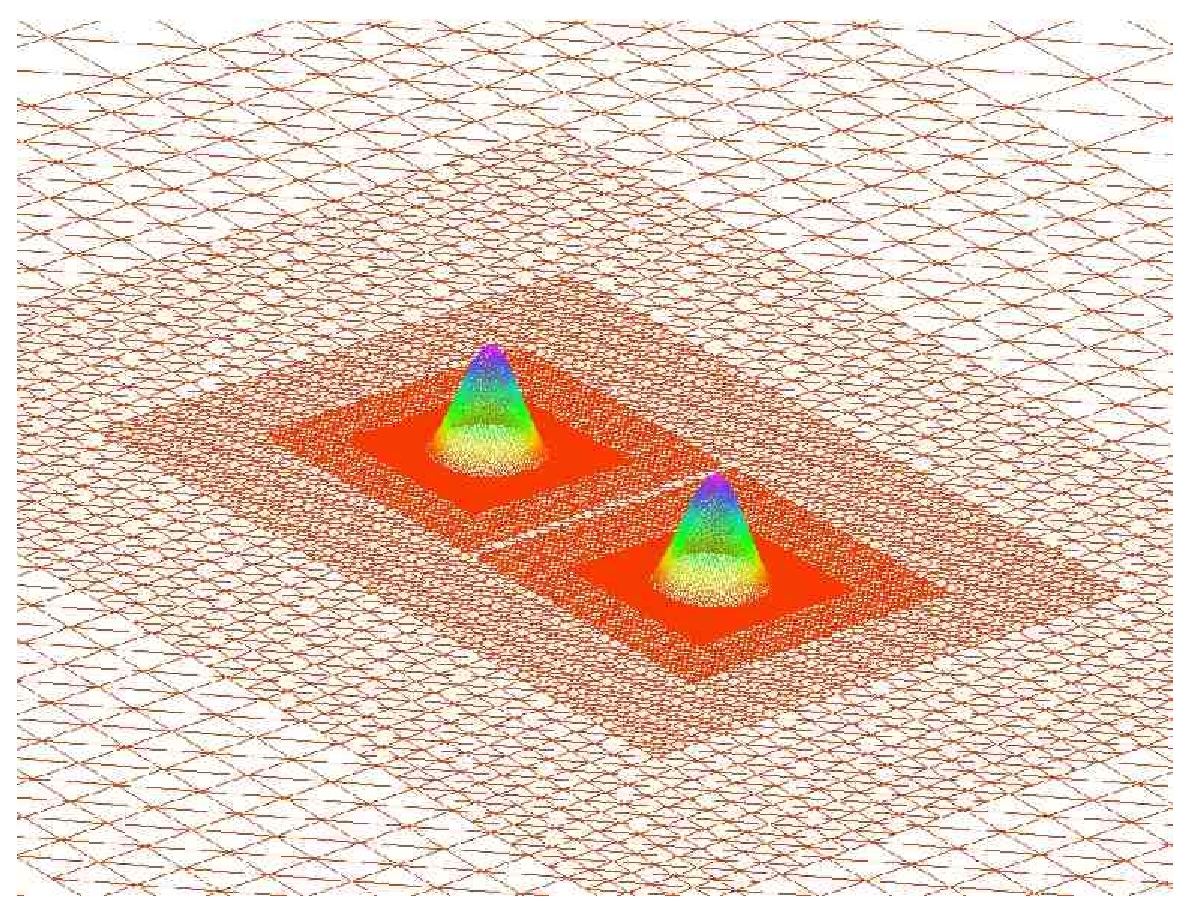
\epsfig{file=figures/grid0.0.ps,height=4.0cm}
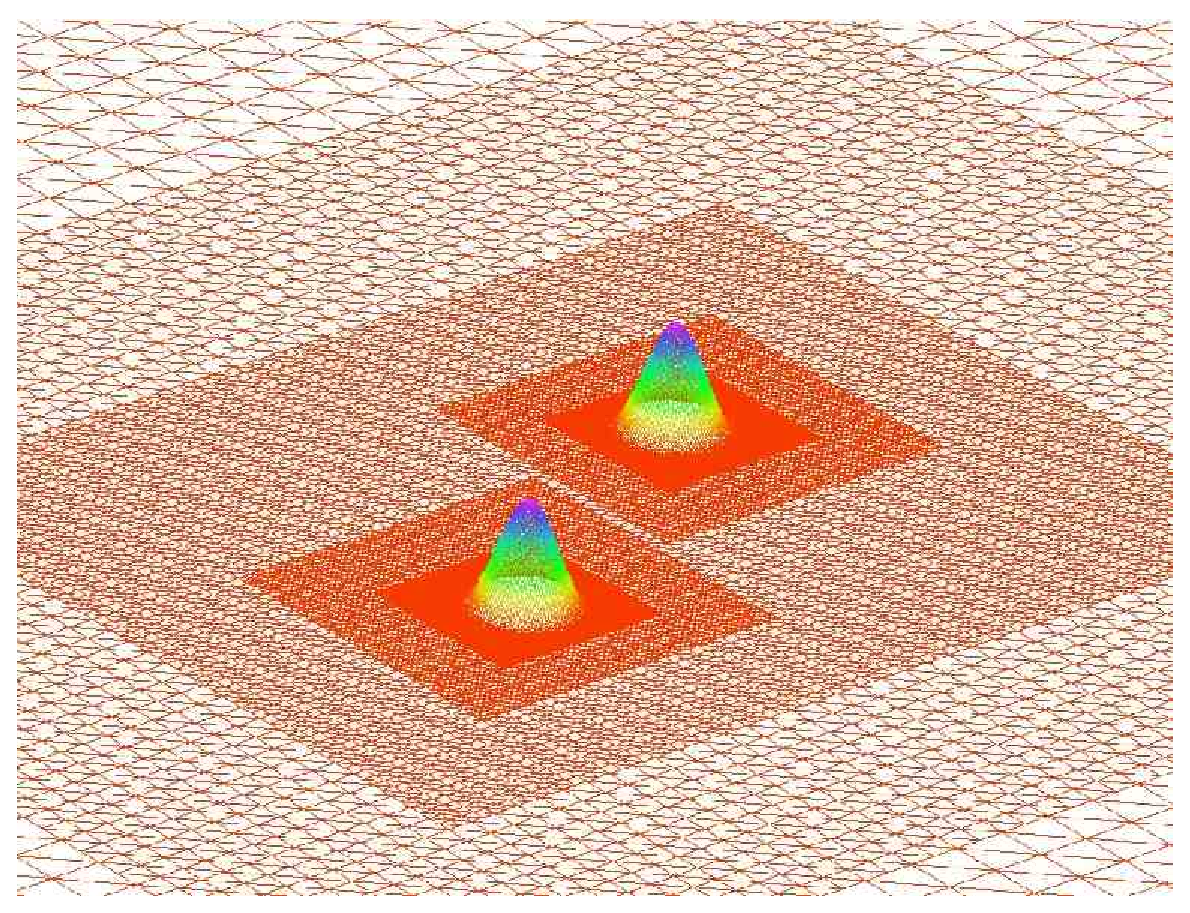
\epsfig{file=figures/grid84.8.ps,height=4.0cm}
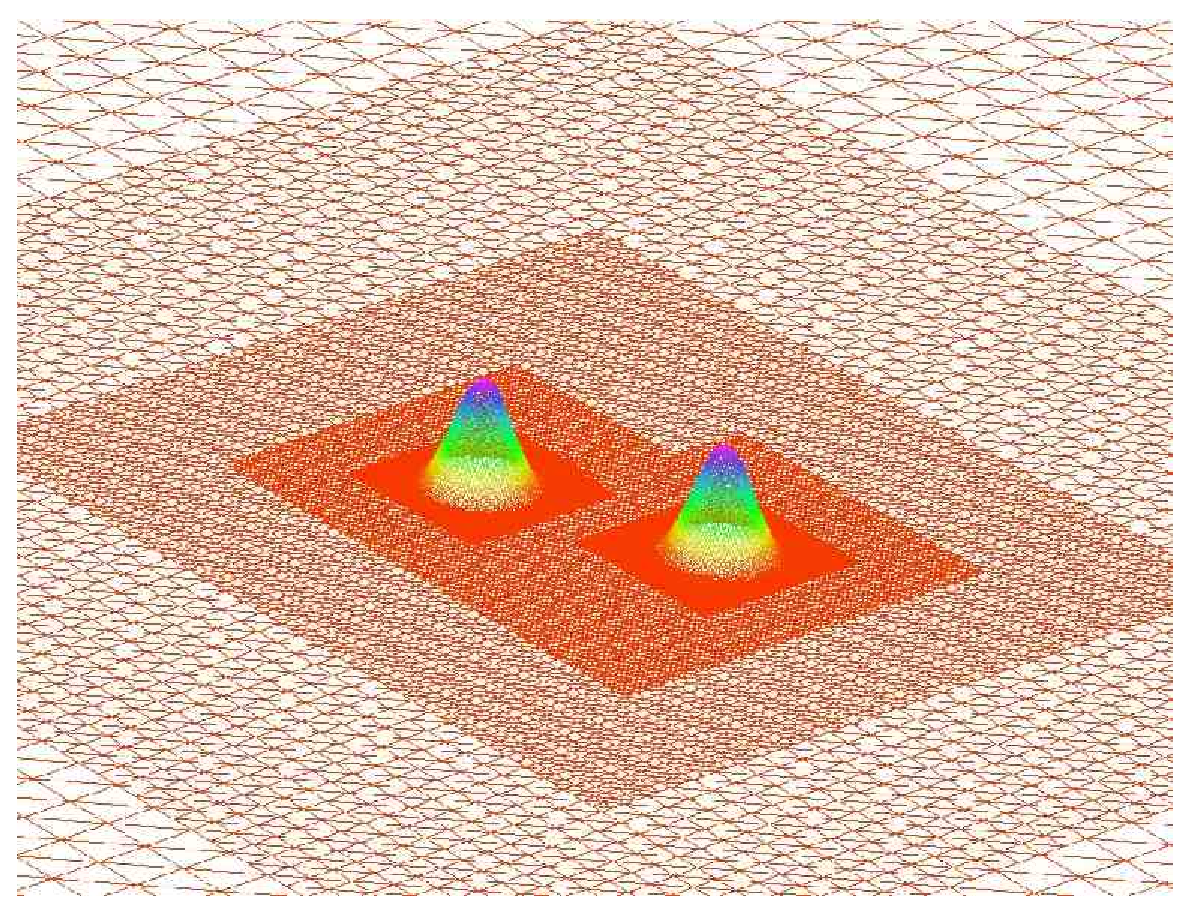
\epsfig{file=figures/grid500.8.ps,height=4.0cm}
\caption{The AMR mesh structure at three different times for the
    pre-merge stage of the simulation with
      a highest resolution of 32 points across each star. This simulation
      was performed using the MPI based HAD toolkit.
    The simulation had seven different resolution levels depending on the relative
error measured locally in the computational domain.  Five of those resolution levels are visible
here.  Simulations were performed on 128 processors.} \label{fig:amr_mesh}
\end{figure}

\begin{figure}
\begin{tabular}{cc}
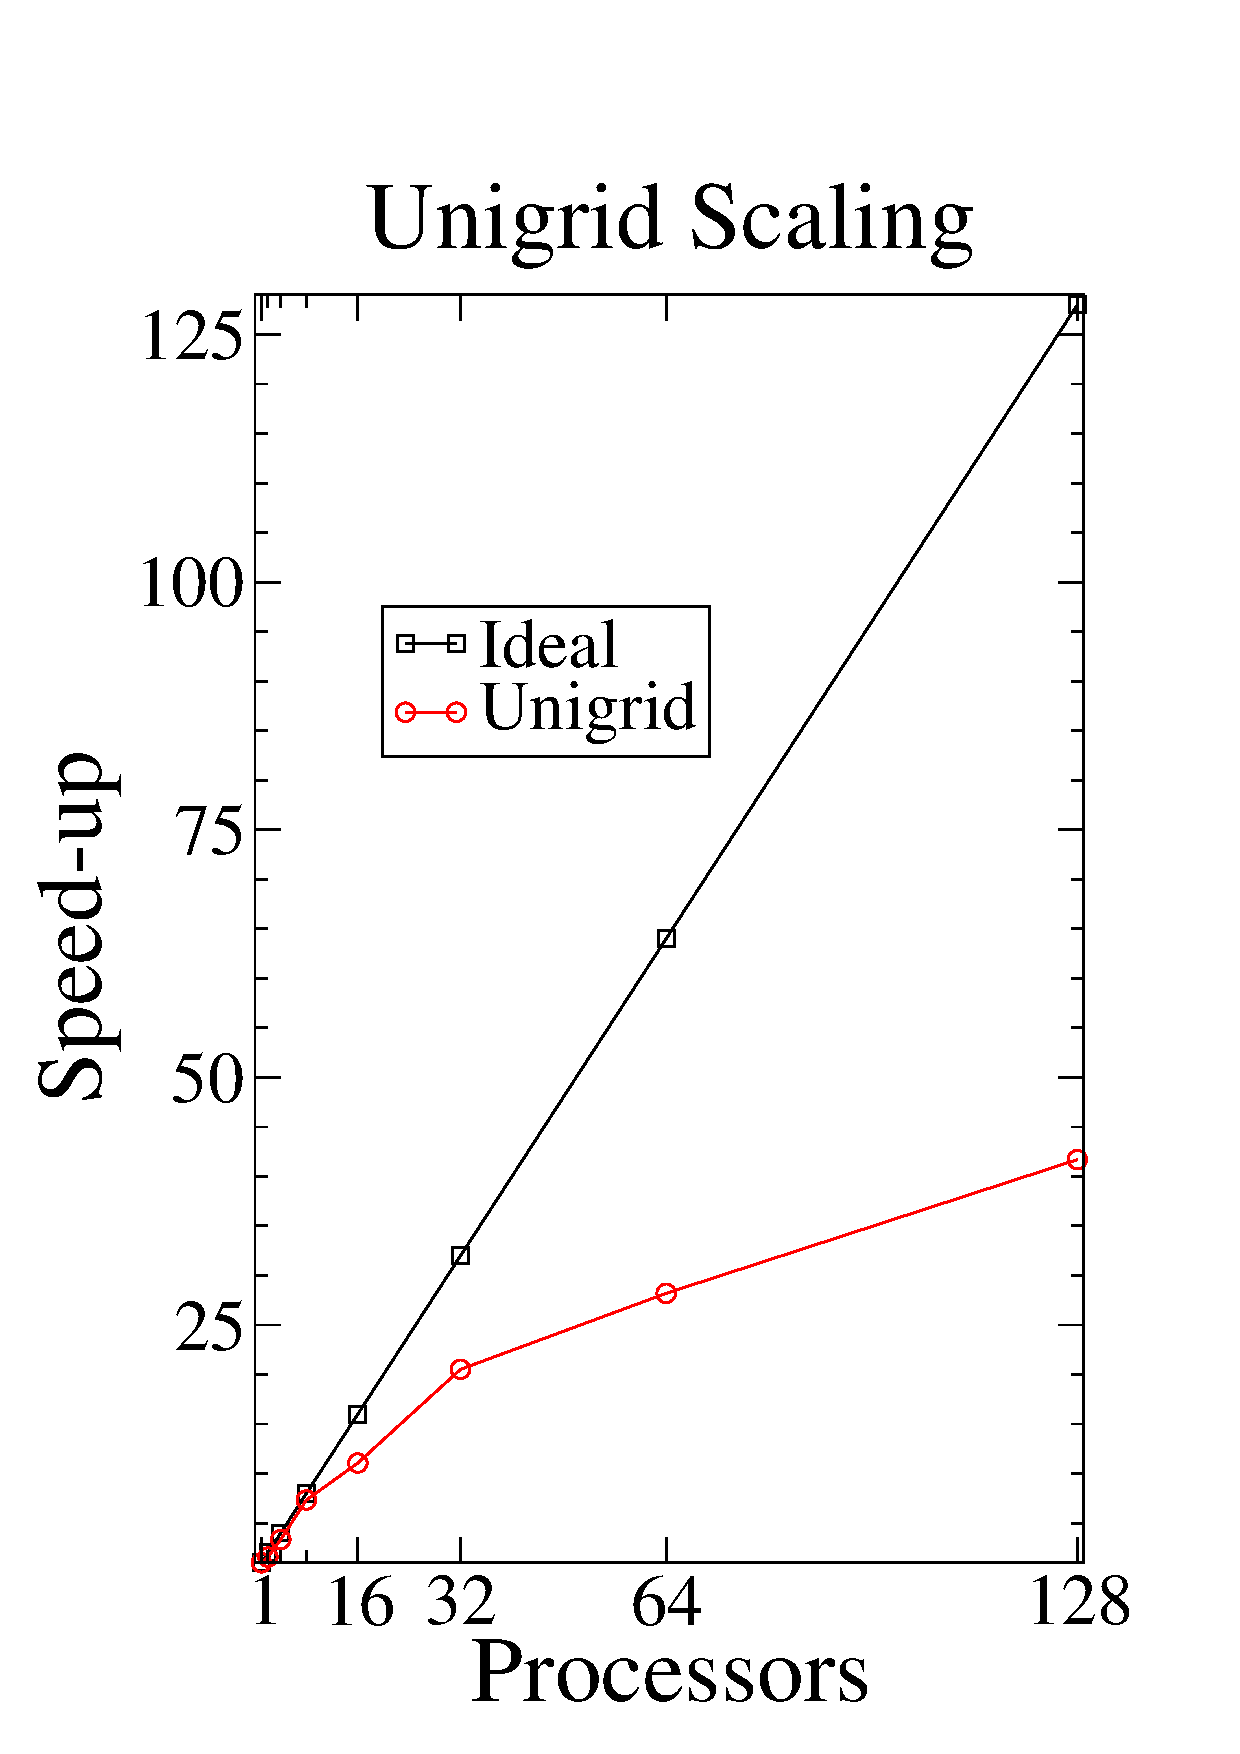
\epsfig{file=figures/strongscale,height=5.5cm} & 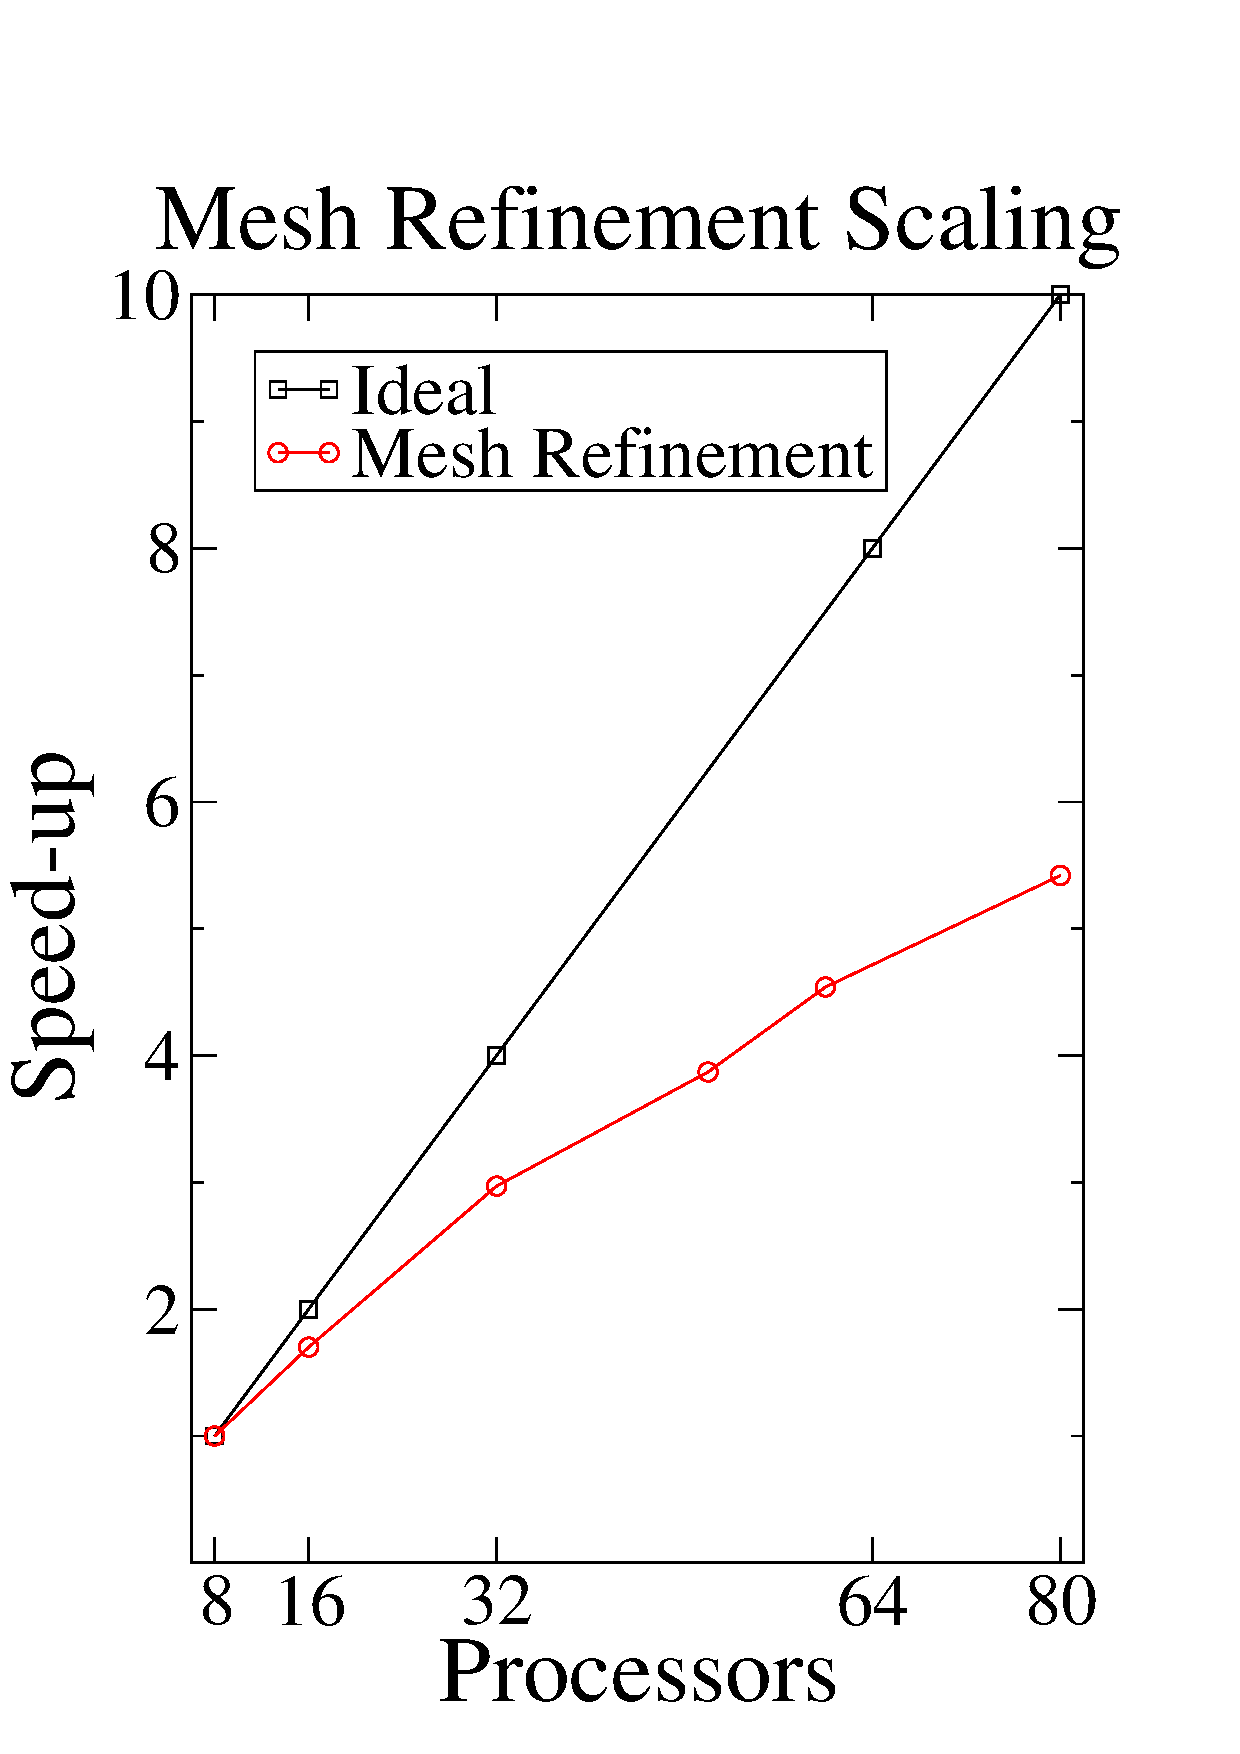
\epsfig{file=figures/amrscale,height=5.5cm} \\
{\bf (a)} & {\bf (b)}
\end{tabular}
\caption{This figure shows strong scaling results for single grid and
 mesh refinement using the MPI based \had\ AMR toolkit.
A spherical blast wave initial dataset wase run for a fixed problem size
as the number of processors is varied.  The left frame shows
the unigrid strong scaling results, and the right frame includes mesh
refinement.  For the unigrid scaling, the data were evolved for 80 iterations,
and the global grid size was $121^3$.  For this problem size, the
communication overhead begins to overshadow the local process computation
on $\geq 64$ processors.  For the mesh refinement scaling,
thirty iterations were performed
on a coarse grid of size $81^3$ and a single level of refinement.
Since the test problem would not fit in memory on a single processor,
speed-up was measured using 8 processors as the base value.
All tests were performed on an Intel Pentium IV 3.0 GHz cluster with Myrinet.}
\label{fig:sphshock-strongscaling}
\end{figure}

\begin{figure}
\begin{tabular}{cc}
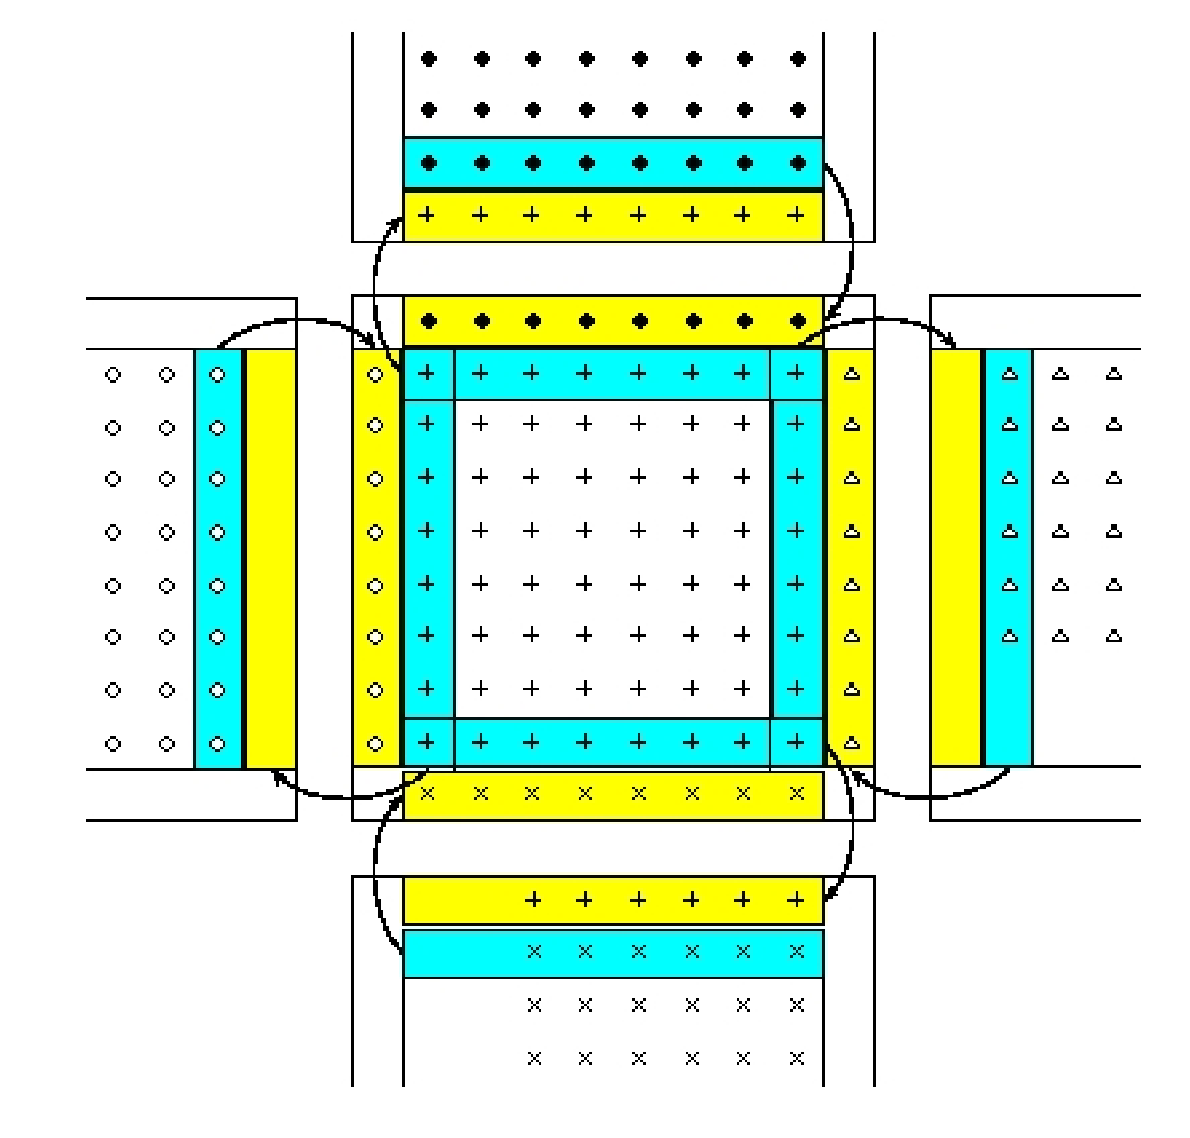
\epsfig{file=figures/communication.ps,height=4.5cm} & 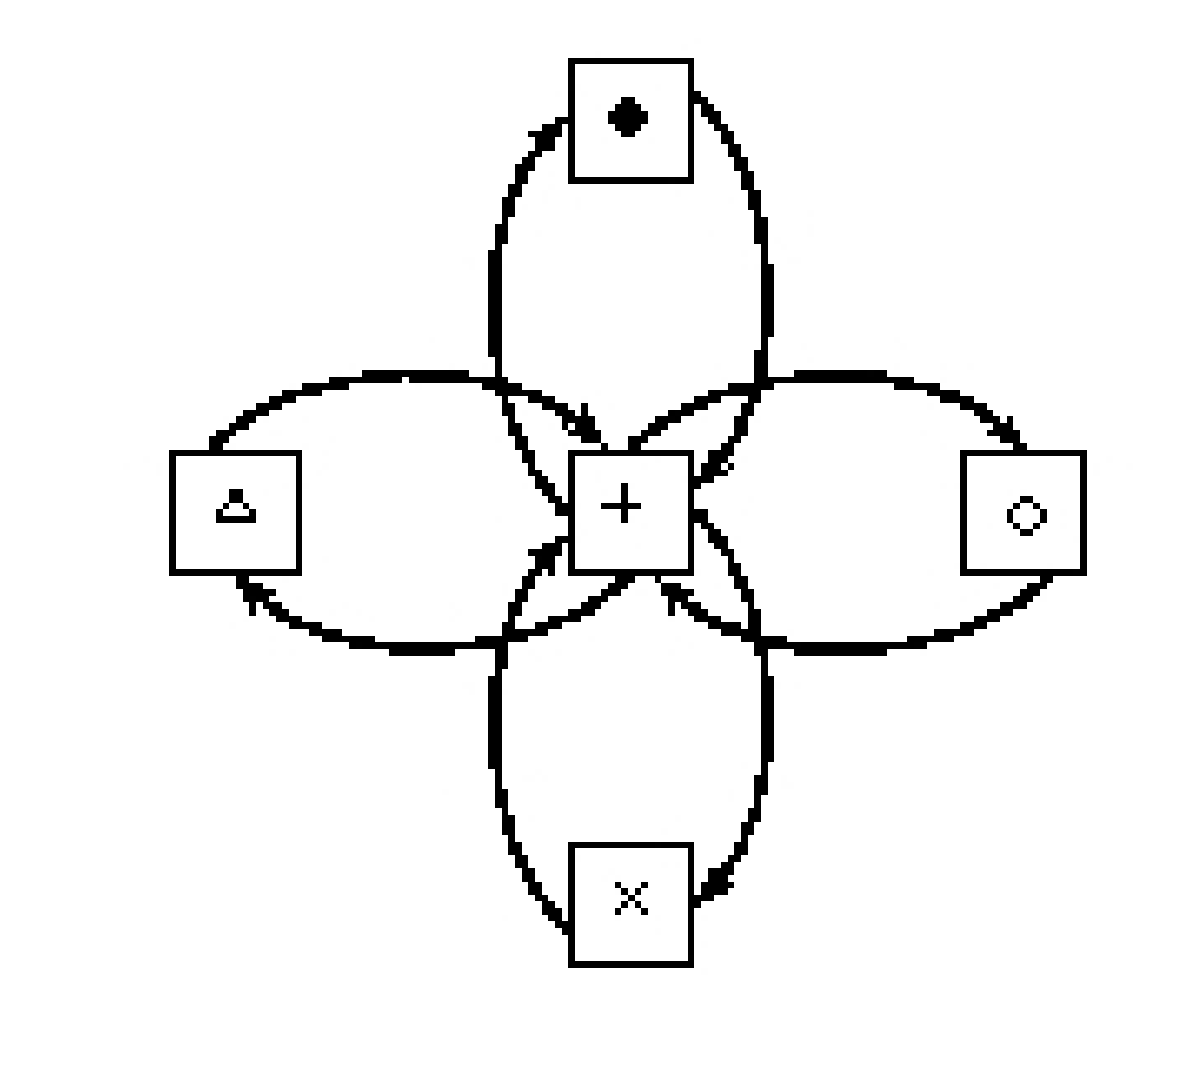
\epsfig{file=figures/granularity.ps,height=3.0cm} \\
{\bf (a)} & {\bf (b)}
\end{tabular}
\caption{Two different approaches to structured mesh based communication: 
(a) 2-D representation of a typical communication pattern for a finite difference
based AMR code.  Large blocks of memory are passed to the user for computation where only
the boundaries of the blocks are communicated among processors.  In this figure, the yellow regions
(frequently referred to as ghostzones) are communicated regions originating from blue zones on 
a distributed memory block as indicated by the arrows.
The current HPX based \had\  approach is seen in (b).  
Here each point is communicated giving the simulation
the smallest granularity possible.  While the amount of communication required in paradigm (b) is 
substantially more than in (a), those communication costs are reduced by the locality
management inherent in HPX.  Paradigm (b) is advantageous for eliminating global
computation barriers.  HPX based \had\ will eventually be capable of both paradigm (a) and (b)
controlled as a runtime parameter so the user can adjust the optimal granularity for a 
particular problem on a particular number of processors.
} \label{fig:granularity}
\end{figure}

\begin{figure}
\epsfig{file=figures/unigrid.ps,height=5.0cm}
\caption{The unigrid mesh structure  
for a 1-D space and time simulation where each node point requires information
from both adjacent neighbors in order to compute a result for the next stage in the simulation.
When the input data (indicated by "{\bf In}") required for operation $F_{0,i}$ to compute a result 
for Stage 0 is available, the computation proceeds.  The $F_{0,i}$ operation can proceed without
waiting for the adjacent operations $F_{0,i-1}$ and $F_{0,i+1}$ to be ready.}
\label{fig:unigrid}
\end{figure}

\begin{figure}
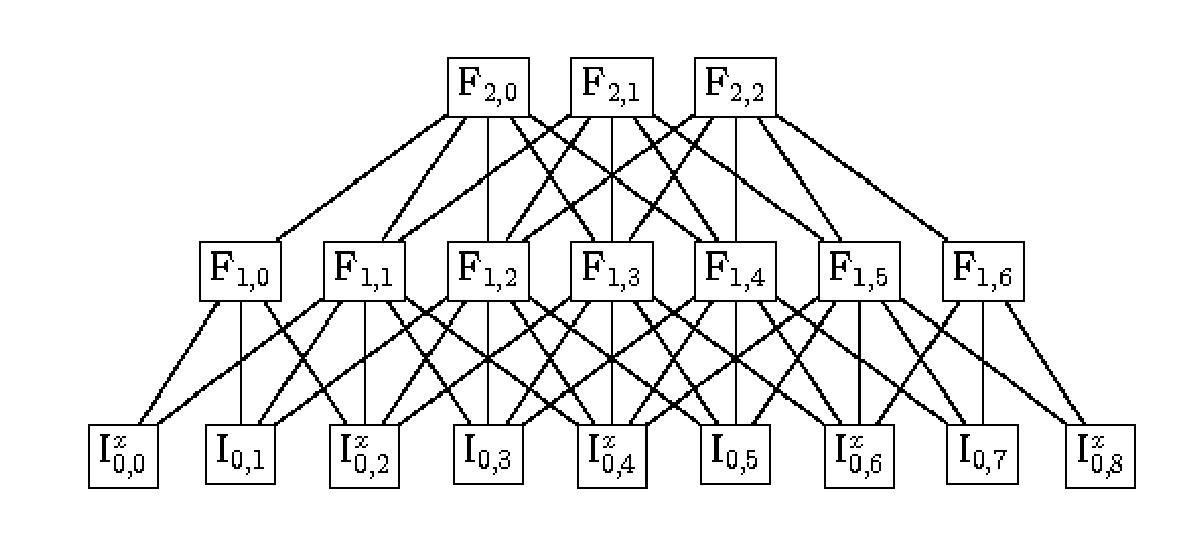
\epsfig{file=figures/tapered.ps,height=5.0cm}
\caption{The left tapered mesh structure.}
\label{fig:tapered}
\end{figure}

%%%%%%%%%%%%%%%%%%%%%%%%%%%%%%%%%%%%%%%%%%%%%%%%%%%%%%%%%%%%%%%%%%%%
%
%   E N D   D O C U M E N T
%
%%%%%%%%%%%%%%%%%%%%%%%%%%%%%%%%%%%%%%%%%%%%%%%%%%%%%%%%%%%%%%%%%%%%
\end{document}

% LocalWords:  circumbinary Shakura Sunyaev 
